\documentclass[]{article}
\usepackage{graphicx}
\graphicspath{ {./images/} }
\usepackage{subcaption}
\usepackage{amsthm}
\usepackage{amsfonts}
\usepackage{amsmath}
\usepackage{amssymb}
\usepackage{ mathrsfs }
\usepackage[ruled,linesnumbered]{algorithm2e}
\newtheorem{mydef}{Definition}[section]
\newtheorem{mytheorem}{Theorem}[section]

%opening
\title{Master Thesis --  Math Formalization}
\author{Kefang Ding} 
\date{9 Nov 2018}

\begin{document}

\maketitle

\hrulefill
\hrulefill 

\begin{abstract}
This article describes the mathematical formalization of the algorithm, which repairs process model by incorporating negative information. The following sections are organized in this way. Section 1 describes the problems to solve. Section 3 introduces formal definitions for dfg-method and adding long-term dependency. Section 4 gives details of the algorithm steps. 
\end{abstract}

\section{Introduction}
The inputs for process model repair include one existing process model, a corresponding event log and a set of KPIs for the data evaluation in event log. After evaluating event log by KPIs, positive and negative labels are assigned on each trace in event log file. 

In state-of-the-art technologies in process mining, only positive traces are used to repair model, while negative information is omitted. In this way, the generated models have low precision. In order to increase the precision, we adapt Inductive Miner algorithm on the base of directly-follows relation of activities. This algorithm, called dfg-algorithm, uses both positive and negative information from event log and generates a model with high fitness. Yet after application, dfg-algorithm cannot discover, change the long-term dependency in the model, so that the model still has less precision. With concept long-term dependency, it describes the dependency between activities, where the execution of one activity affects the execution of another activities later. Later, we investigate problem and propose one algorithm to add long-term dependency constraints in model. 
%% we have the model of Petri net from 

In this article, we propose one algorithm which combines dfg-method and adding long-term dependency programs, to incorporate negative information. The architecture of this model repair algorithm is as shown in Figure \ref{fig:architecture_blackbox}.
\begin{figure}[!h]
	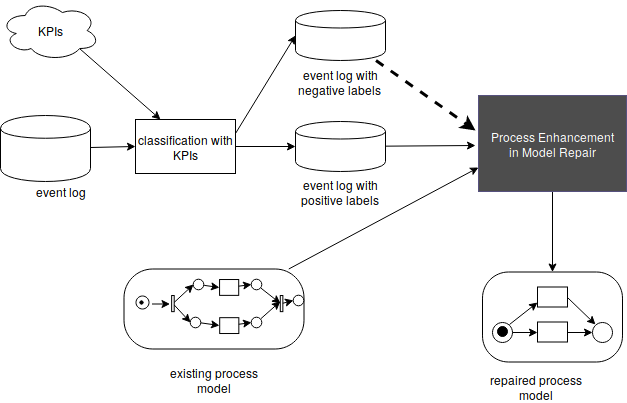
\includegraphics[width=\textwidth]{FD00_approach_blackbox.png} 
	\caption[Model Repair Architecture]{Model Repair Architecture -- \small firstly, event log is divided into positive and negative logs according to KPIs. Later, they are passed as inputs into repair process with existing process model. The output of this process is repaired model.}
	\label{fig:architecture_blackbox}
\end{figure}
%% some explanation about this architecture.

\section{Definitions}
\subsection{Definitions Related To Dfg-Method}
In this part, we provides concepts related to the dfg-method which is based on directly-follows graph. A directly-follows graph as used in \cite{leemans2013discovering}, represents the directly-follows relation of activities in event log. For instance, if there are traces of $\langle ...,A,B,... \rangle$ in event log, one edge (A,B) is added into directly-follows graph. By cutting directly-follows graph under different conditions, Inductive Miner\cite{leemans2013discovering,leemans2014discovering} discovers a process model. Unlike this process, we adapt Inductive Miner to repair model by using existing model, and event log with labels.
 
\begin{mydef}[Cardinality in directly-follows graph]
	Given a directly-follows graph G(L) derived from an event log L, the cardinality of each directly-follows relation in G(L) is defined as:  
	\begin{itemize}
		\item $Cardinality(E(A,B))$ is the frequency of traces with $\langle ...,A,B,... \rangle$. 
		\item Start node A cardinality $Cardinality(Start(A))$ is the frequency of traces with begin node A.
		\item End node B cardinality $Cardinality(End(A))$ is the frequency of traces with end node B.
	\end{itemize}	
\end{mydef}
From the positive and negative event log, we can get directly-follows graphs, respectively $G(L_{pos})$ and $G(L_{neg})$. Each edge of  $G(L_{pos})$ and $G(L_{neg})$ has a cardinality to represent the strength of this directly-follows relation. 
However, when the existing model is transformed into  directly-follows graph $G(L_{ext})$, there is no meaning to assign cardinality on each edge. So we just set 1 to cardinality of each edge. 

%To incorporate all information from  $G(L_pos)$, $G(L_neg)$ and $G(L_ext)$, a data structure is defined directly-follows matrix. 
To incorporate all information from  $G(L_{pos})$, $G(L_{neg})$ and $G(L_{ext})$, we define  weight for each directly-follows relation in graph. 
\begin{mydef}[Weight of directly-follows relation]
	Given a directly-follows graph G(L), the weight of each directly-follows relation is defined as \[ Weight(E(A,B)) = \frac{Cardinality(E(A,B))}{Cardinality(E(A,*))}  \] 
	for start activities A, we have 
	\[ Weight(Start(A)) = \frac{Cardinality(Start(A))}{Cardinality(Start(*))} \]
	Similarly for end activities B, we have
	\[ Weight(End(B)) = \frac{Cardinality(End(B))}{Cardinality(End(*))} \]
	E(A,*) means all edges with source A, E(*,B) means all edges with target B, Start(*) represents all start nodes, and End(*) represents all end nodes.
\end{mydef}
After defining the weights of each directly-follows relation, for each directly-follows relation, there are three weights from $G_{pos}$, $G_{neg}$ and $G_{ext}$. The following strategy assigns new weight to directly-follows relation to new generated directly-follows graph $G_{new}$.
\begin{mydef}[Assign new weights to graph $G_{new}$]
	For one directly-follows relation, there are three weights from $G_{pos}$, $G_{neg}$ and $G_{ext}$, the new weight is \[ Weight(E_{G_{new}}(A,B)) = Weight(E_{G_{pos}}(A,B)) + Weight(E_{G_{ext}}(A,B)) - Weight(E_{G_{neg}}(A,B))\]
		for start activities A, we have 
	\[ Weight(Start_{G_{new}}(A)) = Weight(Start_{G_{pos}}(A)) + Weight(Start_{G_{ext}}(A)) - Weight(Start_{G_{neg}}(A)) \]
	for end activities B, we have
	\[ Weight(End_{G_{new}}(A)) = Weight(End_{G_{pos}}(A)) + Weight(End_{G_{ext}}(A)) - Weight(End_{G_{neg}}(A)) \]
\end{mydef}
After assigning all the weight to directly-follows relation in $G_{new}$, we filter out all directly-follows relation in $G_{new}$ with weight less than 0. 
Then, we transform the $G_{new}$ into process tree for the next stage.

\subsection{Definitions Related To Add Long-term Dependency}
\textit{Example 1} Consider event log L with labels \[L =[\langle A,C,E \rangle^{10,pos}, \langle B,C,D \rangle^{10,pos}, \langle A,C,D \rangle^{10,neg}]. \] $\langle A,C,E \rangle^{10,pos}$ means there are 10 traces $\langle A,C,E \rangle$ labeled as positive in event log. Similarly, $\langle A,C,D \rangle^{10,neg}$ represents there are $\langle A,C,D \rangle$ traces at number 10 in event log which have negative labels. 

After applying the dfg-algorithm, a model as shown in Figure \ref{fig:pn_without_lt_exm01} is discovered. In event log L, B and D has long-term dependency, and A is expected to support only the execution of E, since $<A,C,D>$ is negative and $<A,C,E>$ is positive. However, the model doesn't express those constraints.
\begin{figure}[h!]
	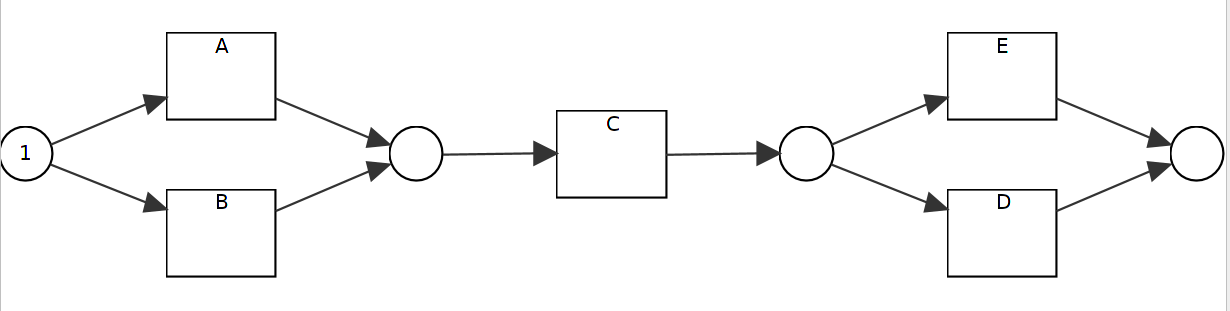
\includegraphics[width=\textwidth]{PN06_Seq_2_xor_notnested.png}
	\caption{Process model generated from dfg-algorithm}
	\label{fig:pn_without_lt_exm01}
\end{figure}
Obviously, long-term dependency relates the choices structure in process model, such as exclusive choice, loop and or structure. Due to the complexity of or structure, only the long-term dependency in exclusive choice and loop structures is considered. 

The inputs for this algorithm are,
\begin{itemize}
	\item Repaired model in process tree
	\item Event log with positive and negative labels
\end{itemize}
The output of this algorithm is: 
\begin{itemize}
	\item Repaired model in petri net with long-term dependency
\end{itemize}

Process tree, as one input for the algorithm, is one common model to interpret process in process mining. It's a block-structured tree. To specify the process tree with respect to long-term dependency, the following definitions are in need. Firstly, the definitions related to tree are reviewed.
\begin{mydef}[Tree]
	Let $ \mathscr{E} $ be a finite set of entities, a tree is a collection of entities called nodes, which are connected by edges. A tree T is,
	\[
	\begin{array}{ rll}
		\circ&t & \mbox{with } t\in \mathscr{E},  \text{t has no outgoing edges}\\
		\circ&t(T_1,T_2,...,T_n) & \mbox{with} t\in \mathscr{E}, i,n\in \mathbb{N}, i \leq n ,T_i\;is\; a\; tree.
	\end{array}
	\]
\end{mydef}
$T_i$ is a child or subtree of $t(T_1,T_2,...,T_n)$, $t(T_1,T_2,...,T_n)$ is one parent of $T_i$, which can be expressed in $P(t(T_1,T_2,...,T_n),T_i)$. The root of tree is the node without any parent; A tree has only one root. A leaf node is the node which has no children nodes.\\
For a node in a tree, its ancestor and descendant are defined as:
\begin{mydef}[Ancestor]
	An ancestor for a node t is a node A in a tree, if 
	\[\text{A is the parent of t or} \]
	\[ \exists t_1,t_2..t_n,n\in \mathscr{E}, i < n, P(A,t_1)\land P(t_i,t_{i+1}) \land P(t_n,t) \]
\end{mydef}
For root, the ancestor is empty, while leaf nodes has no descendants. Except his, for two nodes t and s, if t is the ancestor of s, we have relation Anc(t,s) true. We also define Ancestors(s) as the set of all ancestors of a node s. Similarly, a descendant for a node t is a node s, if t is the ancestor of s, then s is the descendant of node t and Des(s,t) is true; The set of descendants of node t is Descendants(t).
\begin{mydef}[Least Common Ancestor]
	A least common ancestor for node $s$ and node $t$ in a tree is a node n, where 
	\[A(n,s) \land A(n,t) \land \exists! m A(n,m) \land A(m,s) \land A(m,t) \]
\end{mydef}
In process tree, all the leaves are activities in business process, and the middle nodes are operators which represents the relations of all its children nodes\cite{vanderAalst:2016:PMD:2948762,leemans2013discovering}. This paper uses four operators in context of long-term dependency.
\begin{mydef}[Process Tree]
	Let $ A \subseteq \mathbb{A} $ be a finite set of activities with silent transition $\tau \in \mathbb{A}$, $\bigoplus \subseteq \{\rightarrow, \times, \land, \circlearrowright\}$ be the set of process tree operators. 
	\begin{itemize}
		\item $Q=a$ is a process tree with $a\in A$, and 
		\item $Q= \oplus (Q_1 , Q_2 ,.. Q_n)$ is a process tree with $\oplus \in \bigoplus$, and $Q_i$ is a process tree, $i\in{1,2,..,n}, n\in \mathbb{N}$. 
	\end{itemize}
\end{mydef}
Process tree operators represents different block relation of each subtree. Their semantics are standardized from \cite{vanderAalst:2016:PMD:2948762, Buijs2012OnTR} and explained with use of Petri net in Figure \ref{fig:pn_pt_relation}\cite{Buijs2012OnTR}.
\begin{figure}[h!]
 	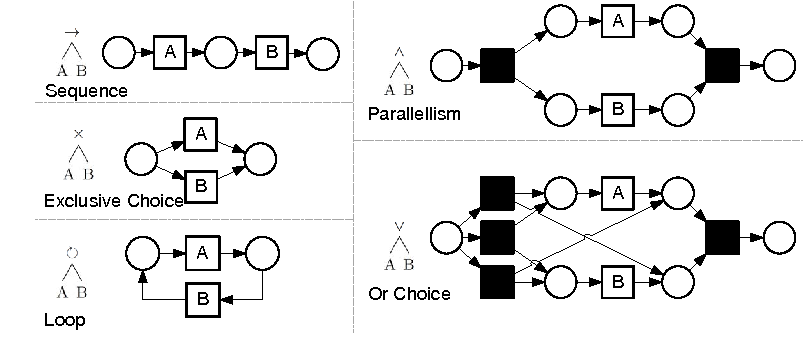
\includegraphics[width=\textwidth]{PT05_Petrinet_PT_Relation.png}
 	\caption{Process Tree With All Operators}
 	\label{fig:pn_pt_relation}
\end{figure}
\begin{mydef}[Operator Semantics] 
	The semantics of operators $\bigoplus \subseteq \{\rightarrow, \times, \land, \circlearrowright, \vee \}$ are,
	\begin{itemize}
		\item if $Q= \rightarrow(Q_1 , Q_2 ,.. Q_n)$, the subtrees have sequential relation and are executed in order of $Q_1,Q_2,..Q_n$
		\item if $Q= \times(Q_1 , Q_2 ,.. Q_n)$,  the subtrees have exclusive choice relation and only one subtree of $Q_1,Q_2,..Q_n$   can be executed.
		\item if $Q= \land (Q_1 , Q_2 ,.. Q_n)$,  the subtrees have parallel relation and $Q_1,Q_2,..Q_n$ they can be executed in parallel.
		\item if $Q= \circlearrowright(Q_1 , Q_2 ,.. Q_n)$,  the subtrees have loop relation and $Q_1,Q_2,..Q_n \; with\; n\geq2$, $Q_1$ is the do-part and is executed at least once, $Q_2,..Q_n$ are redo part and have exclusive relation.
		\item $Q=\vee(Q_1 , Q_2 ,.. Q_n)$, the subtrees have or choice relation and at least one of them executes.
	\end{itemize}
\end{mydef}
\begin{figure}[h!]
	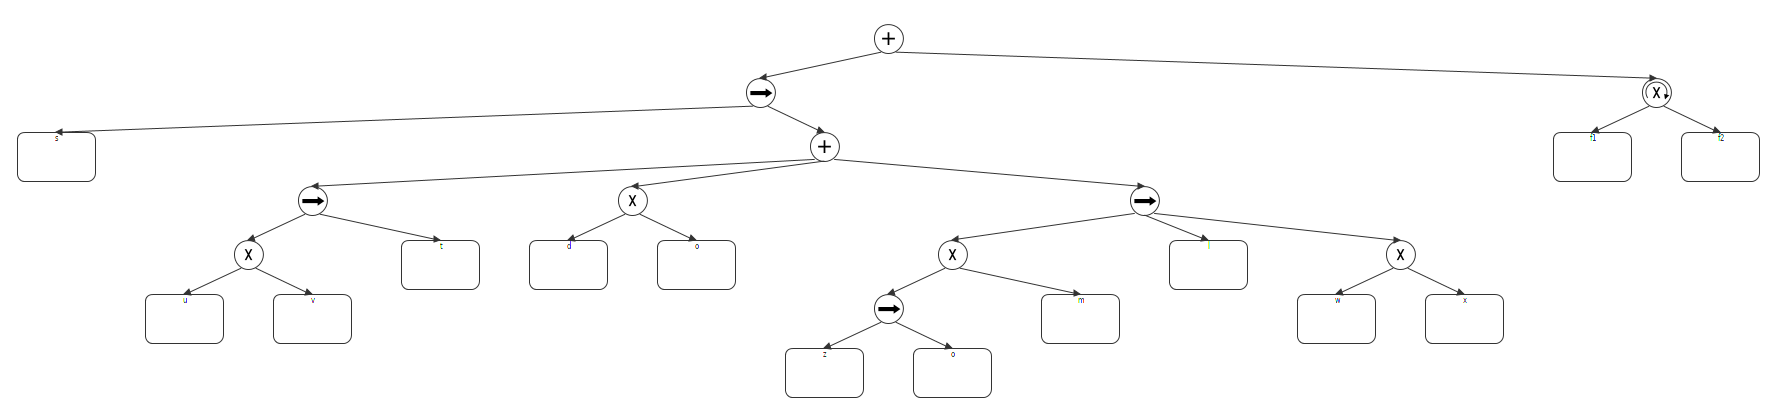
\includegraphics[width=\textwidth]{PT01_Not_Nested_Overview.png}
	\caption{Process Tree With All Operators}
	\label{fig:not_nested_overview}
\end{figure}
An example of process trees is given in the following Figure \ref{fig:not_nested_overview} . It describes a business model, which includes sequential, exclusive choice and parallel relations among the activities. To handle the long-term dependency in the model, exclusive choice, abbr. as xor  and loop are investigated, and several definitions are derived in the next part.
\begin{mydef}[xor branch]
   $Q= \times(Q_1 , Q_2 ,.. Q_n)$, $Q_i$ is one xor branch with respect to Q. For convenience, we use $XORB_{Q_i}$ to represent one xor branch $Q_i$ in xor block, and record it $XORB_{Q_i} \in XOR_{Q}$. For each branch, there exists the begin and end nodes to represent the beginning and end execution of this branch, which is written respectively as Begin($XORB_{Q_i}$) and End($XORB_{Q_i}$).
\end{mydef}
For convenience of analysis, two properties of xor block, purity and nestedness are demonstrated to express the different structures of xor block according to its branches.
\begin{mydef}[XOR Purity and XOR Nestedness] The xor block purity and nestedness are defined as following: \\
	\begin{itemize}
		\item A xor block $XOR_Q$ is pure if and only $\forall XORB_X \in XOR_Q, XORB_X $ is a leaf node. Else, the block is impure.
		\item A xor block $XOR_Q$ is nested if $ \exists XOR_X, Anc(XOR_Q, XOR_X) \rightarrow True  $.
	\end{itemize}
\end{mydef}
In the Figure\ref {fig:xor_nested_branch_variants}, xor block Xor(c1,c2) are pure and not nested, since all the xor branches are leaf node, but xor block Xor(a,Seq(b,Xor(c1,c2))) is impure and nested with Xor(c1,c2). 
\begin{figure}[h!]
	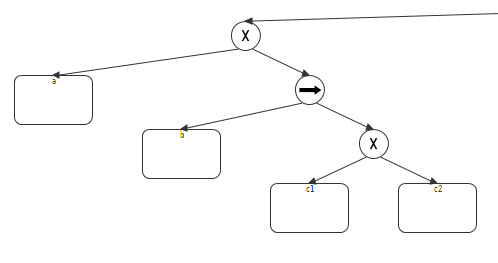
\includegraphics[width=\textwidth]{PT02_xor_nested_and_pure.png}
	\caption{XOR branch variants}
	\label{fig:xor_nested_branch_variants}
\end{figure}
Long-term dependency is associated with choices in xor block, namely each xor branch in xor block. To define it, the following concepts are in need. The first is the order of xor block in sequential structure.
\begin{mydef}[Order of xor block]
	$XOR_A$ is before $xor_B$, written in $XOR_A \prec XOR_B$, if $XOR_A$ is always executed before $xor_B$.  %The least common ancestor of $XOR_A$ and $XOR_B$ is a sequential node. 
\end{mydef}
Consider the model in Figure \ref{fig:not_nested_overview}, we have xor order block, $Xor(Seq(z,o),m) \prec Xor(w,x)$, because the least common ancestor of them is sequential, so they are always executed in an order. However, for Xor(u,v) and Xor(d,o), their least common ancestor is parallel, so they don't have any execution order. If they are in loop as in Figure \ref{fig:xor_in_loop}, we define the xor in do part is before the xor in redo part, namely $Xor(f3,f4) \prec Xor(f6,f7)$.
\begin{figure}[h!]
	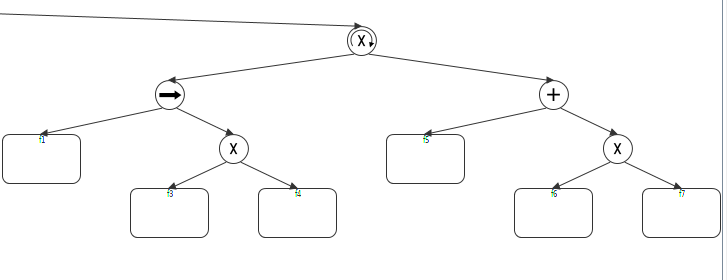
\includegraphics[width=\textwidth]{PT03_xor_in_loop.png}
	\caption{XOR in loop}
	\label{fig:xor_in_loop}
\end{figure}
With the order definition, we introduce the definition for xor pair.
\begin{mydef}[XOR Pair]
	$xor_A$ and $xor_B$ is an xor pair, written in XOR\_Pair($XOR_A, XOR_B$), if $XOR_A \prec XOR_B$.
\end{mydef}
\begin{mydef}[Event Frequency]
	Event Frequency in an event log l is an term $F_{l}(a,freq)$ where a is an activity,$a \in A$  and freq is the happened frequency in integer for event a.
\end{mydef}
In the recursive definition from the above, we can define the xor branch frequency in an event log.
\begin{mydef}[Xor Branch Frequency]
	Xor branch $XORB_X$ frequency in event log l is $F_{l}(XORB_X,freq)$ where $XORB_X$ is an xor branch, and freq is the happened frequency in integer for xor branch $XORB_X$.
\end{mydef}
\begin{mydef}[Supported Connection of Xor branches\footnotemark]
Given an event log, xor branch $XORB_X$ in a xor block $XOR_A$ and $XORB_Y$ in a xor block $XOR_B$ have supported connection over a threshold t, $SC_{l}(XORB_X,XORB_Y,t)$ if and only if
\begin{align*}
 \forall  XORB_X \in XOR_A, XORB_Y \in XOR_B, \exists freq, \\
 F_{l}(XORB_X,freq) \land F_{l}(XORB_Y,freq) \land freq \geq t. 
\end{align*}
\end{mydef}
\footnotetext{here we don't point out the negative instances use. With negative information, it is: $freq(pos) \geq t^{1} \land freq(pos) - freq(neg)\geq t^{2} $}
After introduction of supported connection of xor branches, we can define the long-term dependency. 
\begin{mydef}[Long-term dependency in xor block]
	$XOR_A$ and $XOR_B$ as one xor pair have long-term dependency over an threshold t w.r.t. an event log, $LT(XOR_A, XOR_B, t) $ if and only if 
	\begin{itemize}
		\item there are at least two xor blocks in model, $XOR_A \neq XOR_B \land XOR_A \prec XOR_B$
		\item $\exists XORB_X \in XOR_A, \exists XORB_Y \in XOR_B, \lnot SC_{l}(XORB_X, XORB_Y, t)$. 
	\end{itemize}
\end{mydef}
In this context, we define the long-term dependency between xor branches.
\begin{mydef}[Long-term dependency in xor branches]
	Xor branch $XORB_X$ and $XORB_Y$ have long-term dependency over an threshold t w.r.t. an event log, $LT(XORB_X, XORB_Y, t) $ if and only if  
	\[\exists XORB_X \in XOR_A, \exists XORB_Y \in XOR_B, LT(XOR_A, XOR_B, t) \] \[ \land  SC(XORB_X, XORB_Y, t)  \rightarrow LT(XORB_X, XORB_Y, t).\]	
\end{mydef}
% here we need to define the 
\section{Algorithm Design}
After combining this algorithm, the algorithm is completed to incorporate negative information to repair model as shown in Figure \ref{fig:architecture}.
\begin{figure}
	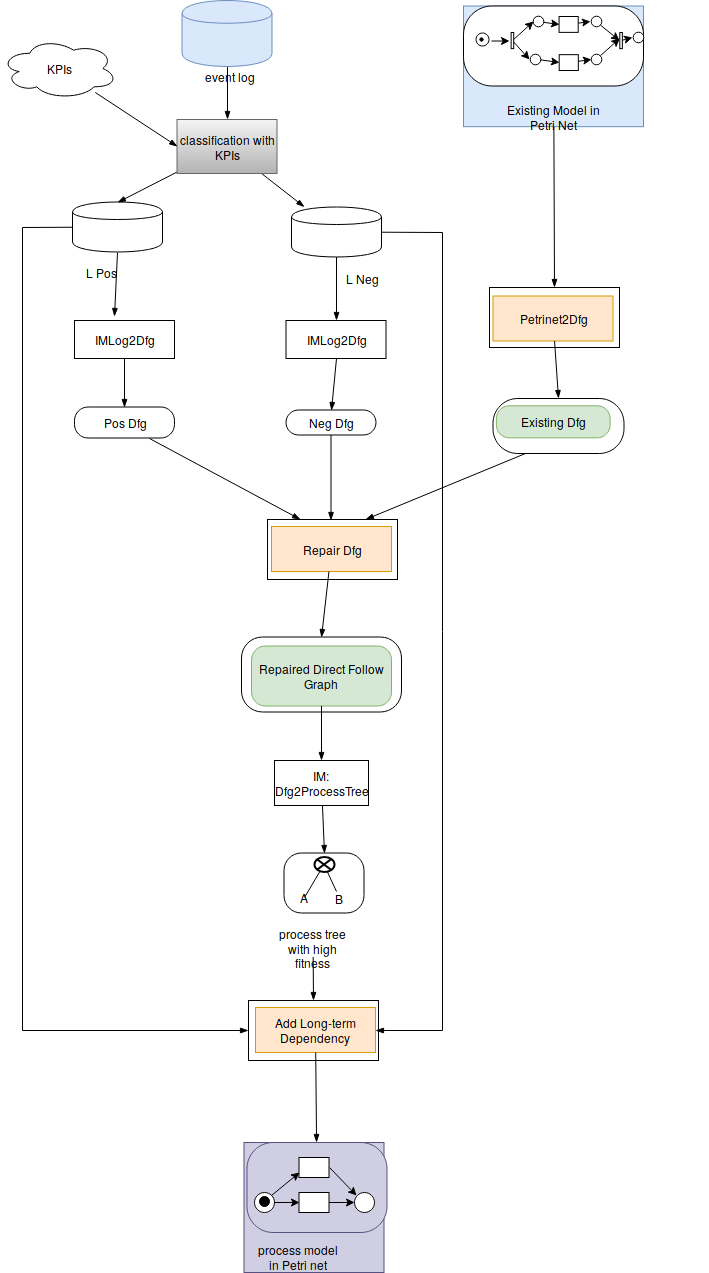
\includegraphics[width=\textwidth, height=\textheight]{FD_architecture_detail_02.png}
	\caption[Model Repair Architecture]{Model Repair Architecture -- \small Rectangles represents processes and output data in eclipse shape, especially customized processes and data are in doubled lattice shape. Input event log and existing model are in blue, KPIs are in cloud. The output is a petri net in purple. }
	\label{fig:architecture}
\end{figure} 
According to the long-term dependency definition, we propose our algorithm to discover long-term dependency. Because the purity, nestedness and its position in process tree, long-term dependency is handled in different situations. However, due to the complexity, the algorithm focuses only on the binary long-term dependency of xor block, which means, we only create xor pair of $XOR_X and XOR_Y$, marked with where 
\[ \exists ! XOR_Z, \: XOR_S \prec XOR_T \rightarrow XOR_S \prec XOR_Z \land XOR_Z \prec XOR_Y \]
The general steps of algorithm is in the following. \\
\begin{algorithm}[H]
	\SetAlgoLined
	\KwResult{Discover Long-term Dependency In Model}
	create a list including all xor pairs in process tree\;
	\While{pair in xor pair list}{
		\If{this pair has no LT dependency}{
			remove this pair from xor pair list\;
		}
	}
	transfer process tree into Petri net\;
	add places in Petri net for every branch pair with long-term dependency\;
	\caption{General steps to add long-term dependency}
\end{algorithm}
We give more details about the each steps in the next parts.
\subsection{Create All XOR Pairs}
Given one process tree with xor blocks, we create XOR pairs in such situations. 
\subsubsection{Sequential XOR Block Without Nested XOR Block}
In this situation, we only consider the model without nested xor block and create xor pair only in sequential order, like in the figure.
%% insert one graph to explain this situation and then create those pairs. 
To get the long-term dependency, the begin and end node in one branch is of importance, it implies the begin and end execution of this xor branch. There are several variants of xor branches as shown in the Figure\ref{fig:xor_branches}.
\begin{figure}[h!]
	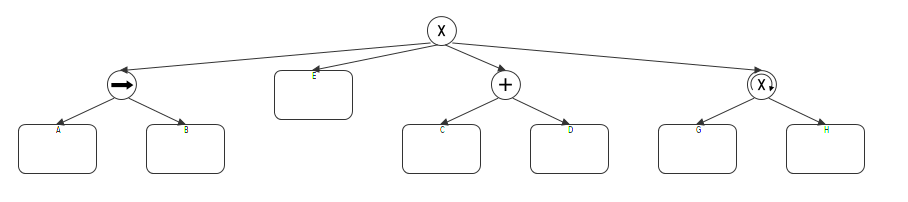
\includegraphics[width=\textwidth]{PT08_xor_branches.png}
	\caption{XOR in loop}
	\label{fig:xor_branches}
\end{figure}
\begin{itemize}
	\item xor branch is a leaf node, the begin node and end node of this branch is this leaf node, like activity E in Fig\ref{fig:xor_branches} written as beginNode = endNode = E;
	\item xor branch is sequential as shown in graph, marked as Seq:(A,B), beginNode = firstChild(Seq)=A, endNode = lastChild(Seq)=B;
	\item xor branch is parallel as shown in graph, marked as And:(C,D), to reduce complexity, we add one sequential node for structure modification; silent activities to the begin and end of sequential structure, and parallel kept in the middle. The xor branch goes back to sequential handle.
	\item xor branch is loop as shown in graph, marked as Loop:(G,H), the similar solution like in parallel, one sequential node is created to keep the loop structure in the middle, two silent activities are divided into the begin and end parts.
\end{itemize}
Or to unify and simply the implementation, for each xor branch, we add implicitly silent activities to mark the beginning and end execution of this xor branch.\\\
\begin{figure}[h]
	\centering
	\begin{subfigure}[b]{\textwidth}
		\centering
		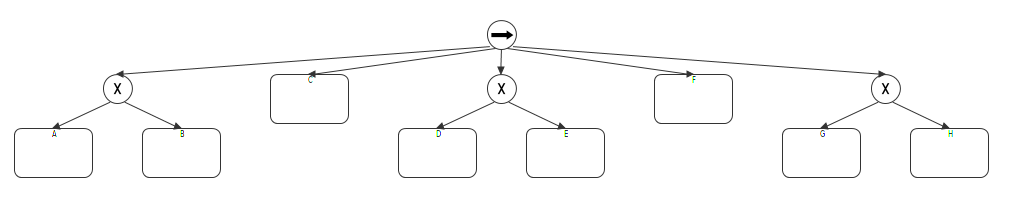
\includegraphics[width=\linewidth]{PT06_Seq_3_xor_notnested.png}
		\caption{Process Tree: sequential relation with 3 xor}
		\label{fig:pt_seq_2_xor}
	\end{subfigure}
	\vfill
	\begin{subfigure}[b]{\textwidth}
		\centering
		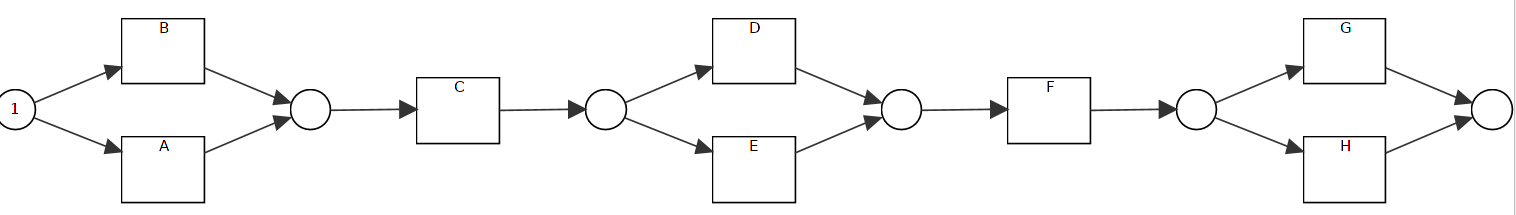
\includegraphics[width=\linewidth]{PN06_Seq_3_xor_notnested.png}
		\caption{Petri net: sequential relation with 3 xor}
		\label{fig:pn_seq_2_xor}
	\end{subfigure}
	\caption{example for xor branch variants in seq}
	\label{fig:seq_situation}
\end{figure}
Two xor blocks exist in the model, they are respectively Xor(A,B), Xor(D,E) and Xor(G,H). After checking the order of xor blocks, we have the direct order $Xor(A,B) \prec Xor(D,E) and Xor(D,E) \prec Xor(G,H)$. So we can create one xor pair Pair(Xor(A,B), Xor(D,E)) and Pair(Xor(D,E), Xor(G,H)).
\subsubsection{Sequential XOR Block With Nested XOR Block}
For the model with nested xor block like Xor:(a,Seq:(b,Xor:(c1,c2))) in Figure\ref{fig:pt_seq_nested} , the nested block needs a redefinition for its branch. 
\begin{itemize}
	\item If one of its xor branches contains no xor block, this branch is kept.
	\item if one xor branch has xor block, called sub xor block, all branches without xor block in the sub xor block should be added to the nested block. 
\end{itemize}
\begin{figure}[h!]
	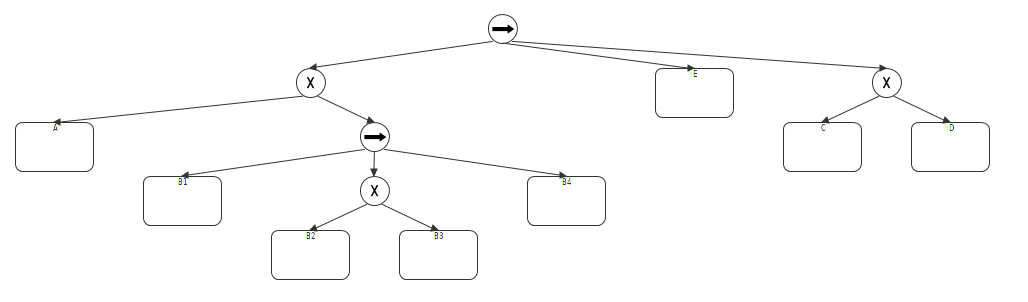
\includegraphics[width=\textwidth]{PT09_seq_xor_nested.png}
	\caption{Sequential nested xor blocks}
	\label{fig:pt_seq_nested}
\end{figure}
So, in the model given by Figure \ref{fig:pt_seq_nested}, for xor block  Xor(A,Seq(B1,Xor(B2,B3),B4)), it has one branch A without xor block, A is therefore kept;  Xor(B2,B3) is nested in Xor(A,Seq(B1,Xor(B2,B3),B4)). 

To create xor pair, we need to put the branches B2 and B3 in the same level of A. It implies that Xor(A,Seq(B1,Xor(B2,B3),B4)) has three real xor branches, which are A, B2 and B3. This procedure is called nested xor block folding. After all xor block is folded, we have two effective xor block, Xor(C,D) and Xor(A,B2,B3) and one pair of them is created, namely Pair(Xor(A,B2,B3), Xor(C,D)).
\subsubsection{Parallel XOR Block}
Given a model with xor blocks in parallel relation and event log which supports long-term dependency, we need to add long-term dependency on the model. There are some situations.
\begin{itemize}
	\item in each parallel branch, there exists one xor block, long-term pattern is one xor branch decides the choices of another xor
	\item in parallel branch, there exist more than one xor block
	\item xor block in parallel branch is nested
\end{itemize}
\begin{figure}[h]
	\centering
	\begin{subfigure}[b]{\textwidth}
		\centering
		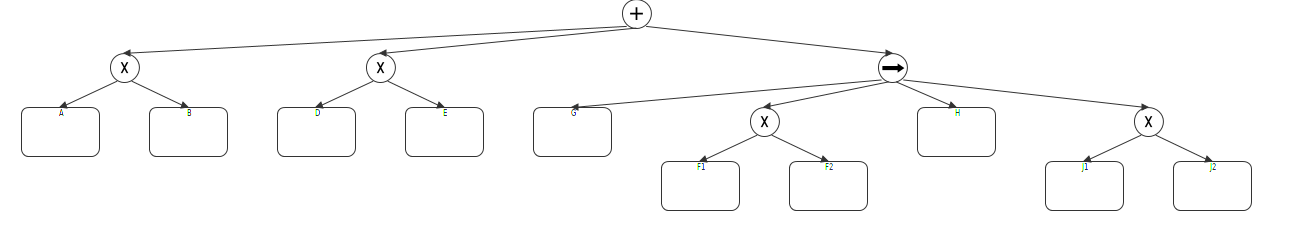
\includegraphics[width=\linewidth]{PT07_And_4_xor_notnested.png}
		\caption{Process Tree: parallel relation with 3 xor}
		\label{fig:pt_and_4_xor}
	\end{subfigure}
	\vfill
	\begin{subfigure}[b]{\textwidth}
		\centering
		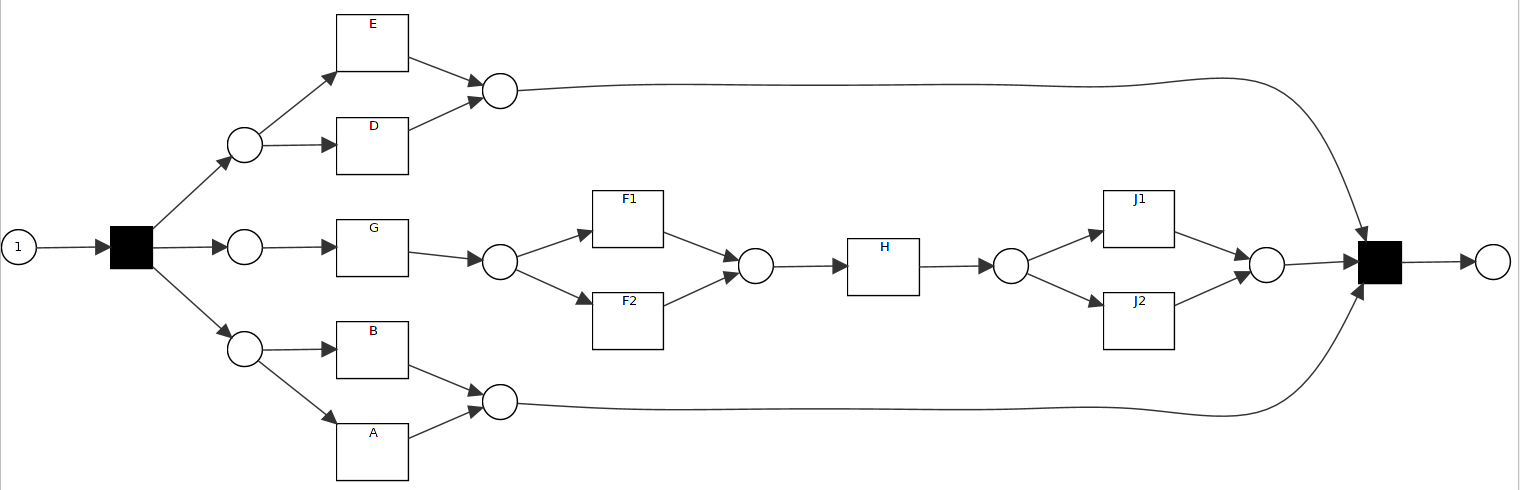
\includegraphics[width=\linewidth]{PN07_And_4_xor_notnested.png}
		\caption{Petri net: parallel relation with 3 xor}
		\label{fig:pn_and_4_xor}
	\end{subfigure}
	\caption{example parallel relation}
	\label{fig:and_situation}
\end{figure}
%% we still need to analyze it, but how to deal with it?? 
\subsubsection{Loop XOR Block}
Long-term dependency divers in loop block as listed below. 
\begin{itemize}
	\item one xor before loop block, several choices for redo part in loop block
	\item one xor after loop block, several choices for redo part
	\item one xor before loop block, xor in do part of loop block
	\item one xor after loop block, xor in do part of loop block
	\item one xor before loop block, xor in redo part of loop block
	\item one xor after loop block, xor in redo part of loop block
	\item xor in loop block do and redo part
	\item one xor before loop, xor in do part and redo part
	\item one xor after loop, xor in do part and redo part
\end{itemize}

\begin{align}
<A, L_{1}^{*} || L_{2}^{*} || E> \\
<B, L_{1}^{*} || L_{2}^{*} || E>
\end{align}
\subsection{Check if the pair has LT Dependency}
After getting all the xor pairs from the model, we check if the pair has long-term dependency with corresponding event log.


\subsection{Transfer Process Tree into Petri Net}
By using already existing application, the process tree is transferred into Petri net without long-term dependency connection. The silent nodes from the last step are also shown in the Petri net as silent transitions.
However, if we discover the long-term dependency directly on the Petri net, we don't need the process tree transformation. In this article, the steps are quite detailed;; But the definitions are general enough for design. 
\subsection{Add Long-term dependency}
In Petri net, long-term dependency is addressed by adding extra places and silent transitions in xor pair.  
% one figure is in need to describe this% 
\begin{algorithm}
	\SetAlgoLined
	Add places after xor join structure \;
		\ForEach{xor branch in xor pair}{
			add one place after its branch end node}    
	Add places before xor split structure\;
	Add silent transition to connect places\;
	\caption{Add long-term dependency in xor pair}
\end{algorithm}
\subsubsection{Sequential}

\subsubsection{Parallel}

\subsubsection{Loop}

\bibliography{bibtex2ref.bib}
\bibliographystyle{ieeetr}
\end{document}
